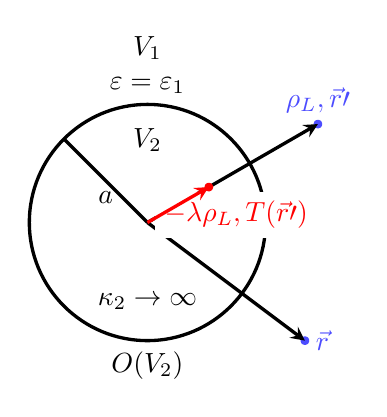
\begin{tikzpicture}[line width = 1.2pt, line join=round,>=stealth]
	\filldraw [color=blue!70] (30:2.5) circle (1pt) node[above] {$\rho_L, \vec{r}\prime $};
	\filldraw [color=blue!70] (2,-1.5) circle (1pt) node[right] {$\vec{r} $};
	\draw [-stealth] (0,0) -- (30:2.5);
	\draw [-stealth] (0,0) -- (2,-1.5);
	\draw (0,0) circle (1.5);
	\draw (0,0) -- (135:1.5);
	\draw (135:0.75 ) node[below] {$a$};

	\draw (0,-1.5) node [below] {$O(V_2)$};
	\draw(0,1.05) node {$V_2$};
	\draw(0,-1) node{$\kappa_2 \to \infty$};
	\draw(0,2.0) node[align=center] {$V_1$\\$\varepsilon=\varepsilon_1$};
	\draw [color=red] (20:1.2) node[below, fill=white] {$-\lambda \rho_L, T(\vec{r}\prime )$};

	\draw [-stealth,color=red] (0,0) -- (30:0.9);
	\filldraw [color=red] (30:0.9) circle (1pt);
\end{tikzpicture}